% TikZ helpers — confusion matrix uses \CmTN, \CmFP, \CmFN, \CmTP from values_*.tex

\newcommand{\TikzConfusionMatrix}{%
  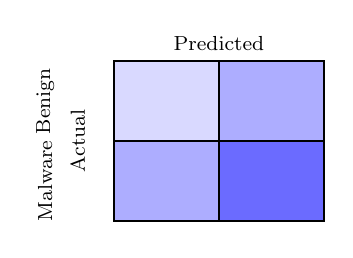
\begin{tikzpicture}[scale=0.92, transform shape,
    font=\small,
    cell/.style={minimum width=1.35cm, minimum height=1.0cm, align=center, inner sep=2pt},
    lbl/.style={font=\footnotesize, align=center},
  ]
  \node[lbl] at (1.45, 2.45) {Predicted};
  \node[lbl] at (0.725, 2.05) {Benign};
  \node[lbl] at (2.175, 2.05) {Malware};
  \node[lbl, rotate=90] at (-0.5, 1.1) {Actual};
  \node[lbl, rotate=90] at (-0.95, 1.65) {Benign};
  \node[lbl, rotate=90] at (-0.95, 0.55) {Malware};
  \fill[blue!15] (0,1.1) rectangle (1.45,2.2);
  \fill[blue!32] (1.45,1.1) rectangle (2.9,2.2);
  \fill[blue!32] (0,0) rectangle (1.45,1.1);
  \fill[blue!58] (1.45,0) rectangle (2.9,1.1);
  \node[cell, font=\small\bfseries] at (0.725, 1.65) {\CmTN};
  \node[cell, font=\small\bfseries] at (2.175, 1.65) {\CmFP};
  \node[cell, font=\small\bfseries] at (0.725, 0.55) {\CmFN};
  \node[cell, font=\small\bfseries] at (2.175, 0.55) {\CmTP};
  \draw[thick] (0,0) rectangle (2.9,2.2);
  \draw (1.45,0) -- (1.45,2.2);
  \draw (0,1.1) -- (2.9,1.1);
  \end{tikzpicture}%
}

% Map raw count to y (cm); axis spans [ymin, ymax] on log10 scale, plotted height \plotH cm.
\newcommand{\TikzCountY}[4]{%
  \pgfmathsetmacro{#4}{(ln(max(#1,1))/ln(10) - ln(max(#2,1))/ln(10)) / (ln(max(#3,1))/ln(10) - ln(max(#2,1))/ln(10))}%
}

\newcommand{\TikzLogStrip}[6]{%
  % #1=x centre, #2=colour, #3=macro with comma list, #4=ymin #5=ymax #6=plot height (cm)
  \foreach \v [count=\i] in #3 {
    \TikzCountY{\v}{#4}{#5}{\yraw}
    \pgfmathsetmacro{\y}{\yraw * #6}
    \pgfmathsetmacro{\dx}{mod(\i-1,2)==0 ? 0.08 : -0.08}
    \fill[#2] (#1+\dx,\y) circle (1.6pt);
  }%
}

\newcommand{\TikzLogAxis}[5]{%
  % #1=x0 #2=x1 #3=ymin #4=ymax #5=plot height (cm)
  \foreach \t/\lbl in {2/100,3/1k,4/10k,5/100k} {
    \pgfmathparse{and(10^\t >= #3, 10^\t <= #4)}
    \ifnum\pgfmathresult=1
      \TikzCountY{10^\t}{#3}{#4}{\yraw}
      \pgfmathsetmacro{\y}{\yraw * #5}
      \draw[gray!55] (#1,\y) -- (#2,\y);
      \node[font=\footnotesize, anchor=east] at (#1-0.08,\y) {\lbl};
    \fi
  }%
}

\newcommand{\TikzTriageBars}[1]{%
  % #1 = max count for bar width scaling
  \pgfmathsetmacro{\barW}{9.2/max(#1,1)}
  \foreach \lbl/\cnt [count=\i] in \BarRows {
    \pgfmathsetmacro{\y}{(\i-1)*0.95}
    \draw[fill=benignblue!75, draw=black!60, line width=0.3pt]
      (0,\y) rectangle ({\cnt*\barW},\y+0.72);
    \node[anchor=west, font=\small] at (0.14,\y+0.36) {\lbl};
    \node[anchor=east, font=\small\bfseries] at ({\cnt*\barW}-0.14,\y+0.36) {\cnt};
  }%
}
